\chapter{Results}
This chapter should encompass your data analysis and findings. Additionally, include relevant tables, figures, and citations to support your results and interpretations. Here is a suggested list of topics to discuss:
\section{Interface Comparison}
During the development of this project, various experiments were conducted to optimize the performance of a quantum molecular simulator. In this context, the choice of the interface for calculating cost functions is crucial, as these functions must be optimized to obtain the optimal state and geometry of each molecule. Typically, the \textit{JAX} interface is the most widely used due to its GPU acceleration capabilities, which generally provide greater efficiency and speed in searching for the minimum of the cost function.

However, when comparing two identical implementations—varying only the calculation interface—we observed a surprising result: the \textit{JAX}-based interface, which was executed on a GPU, was slower than the \textit{autograd}-based interface, which ran on a CPU. To confirm that this was not a coding error, we repeated the experiments on different machines, obtaining the same result. For this reason, we decided to continue with the \textit{autograd} interface due to its greater speed in our specific implementation.

\subsection{Optimization and Timing Logging}
To verify the performance differences between both interfaces, the same optimization was executed while varying only the interface. During these simulations, the execution times of the different functions in the code were recorded, with their values shown in Table~\ref{tab:comparison_gd}.

\begin{table}[H]
  \centering
  \scriptsize
  \resizebox{\textwidth}{!}{%
  \begin{tabular}{lcccccc}
  \toprule
  \textbf{Function} & 
  \textbf{[\texttt{Li}, \texttt{H}] \_autograd\_GD} & 
  \textbf{[\texttt{Li}, \texttt{H}] \_jax\_GD} & 
  \textbf{[\texttt{O}, \texttt{H}, \texttt{H}] \_autograd\_GD} & 
  \textbf{[\texttt{O}, \texttt{H}, \texttt{H}] \_jax\_GD} & 
  \textbf{[\texttt{H}, \texttt{H}] \_autograd\_GD} & 
  \textbf{[\texttt{H}, \texttt{H}] \_jax\_GD} \\
  \midrule
  Iteration 1  & 1246.7627 & 6251.3362 & 6942.21696 & 39003.89009 & 14.6908 & 40.5485 \\
  Iteration 2  & 1244.0321 & 6284.9812 & 6935.09353 & 40652.7751  & 14.7824 & 36.2979 \\
  Iteration 3  & 1247.4399 & 6348.2470 & 6920.68571 & 40386.29868 & 14.9931 & 38.6236 \\
  Iteration 4  & 1245.7256 & 6351.6437 & 6942.60873 & 40128.31419 & 15.0694 & 39.1362 \\
  Iteration 5  & 1244.8591 & 6349.5099 & 6965.70663 & 40657.74473 & 15.1512 & 40.6186 \\
  \midrule
  \textbf{Total Time} & 6228.8195 & 31585.7475 & 34706.3116 & 200829.0866 & 74.6870 & 195.2551 \\
  \textbf{build\_hamiltonian} & 29.1349   & 30.3407  & 78.4744   & 85.7532   & 0.4934   & 0.5329  \\
  \textbf{compute\_operator\_gradients} & 1533.0319 & 17497.4381 & 12563.3726 & 113792.7167 & 0.6313   & 11.9006 \\
  \textbf{update\_parameters\_and\_coordinates} & 4666.6385 & 14056.6795 & 22064.4153 & 86946.6021 & 73.5594 & 182.5271 \\
  \bottomrule
  \end{tabular}%
  }
  \caption{Execution times for different molecules and interfaces using \textit{Gradient Descent}.}
  \label{tab:comparison_gd}
\end{table}

Figure~\ref{fig:time_iterations} shows how the execution time evolves over the iterations for each molecule and type of interface. It is evident that, in all cases, the \textit{autograd}-based interface offers lower computation times than the \textit{JAX}-based interface.

\begin{figure}[H]
  \centering
  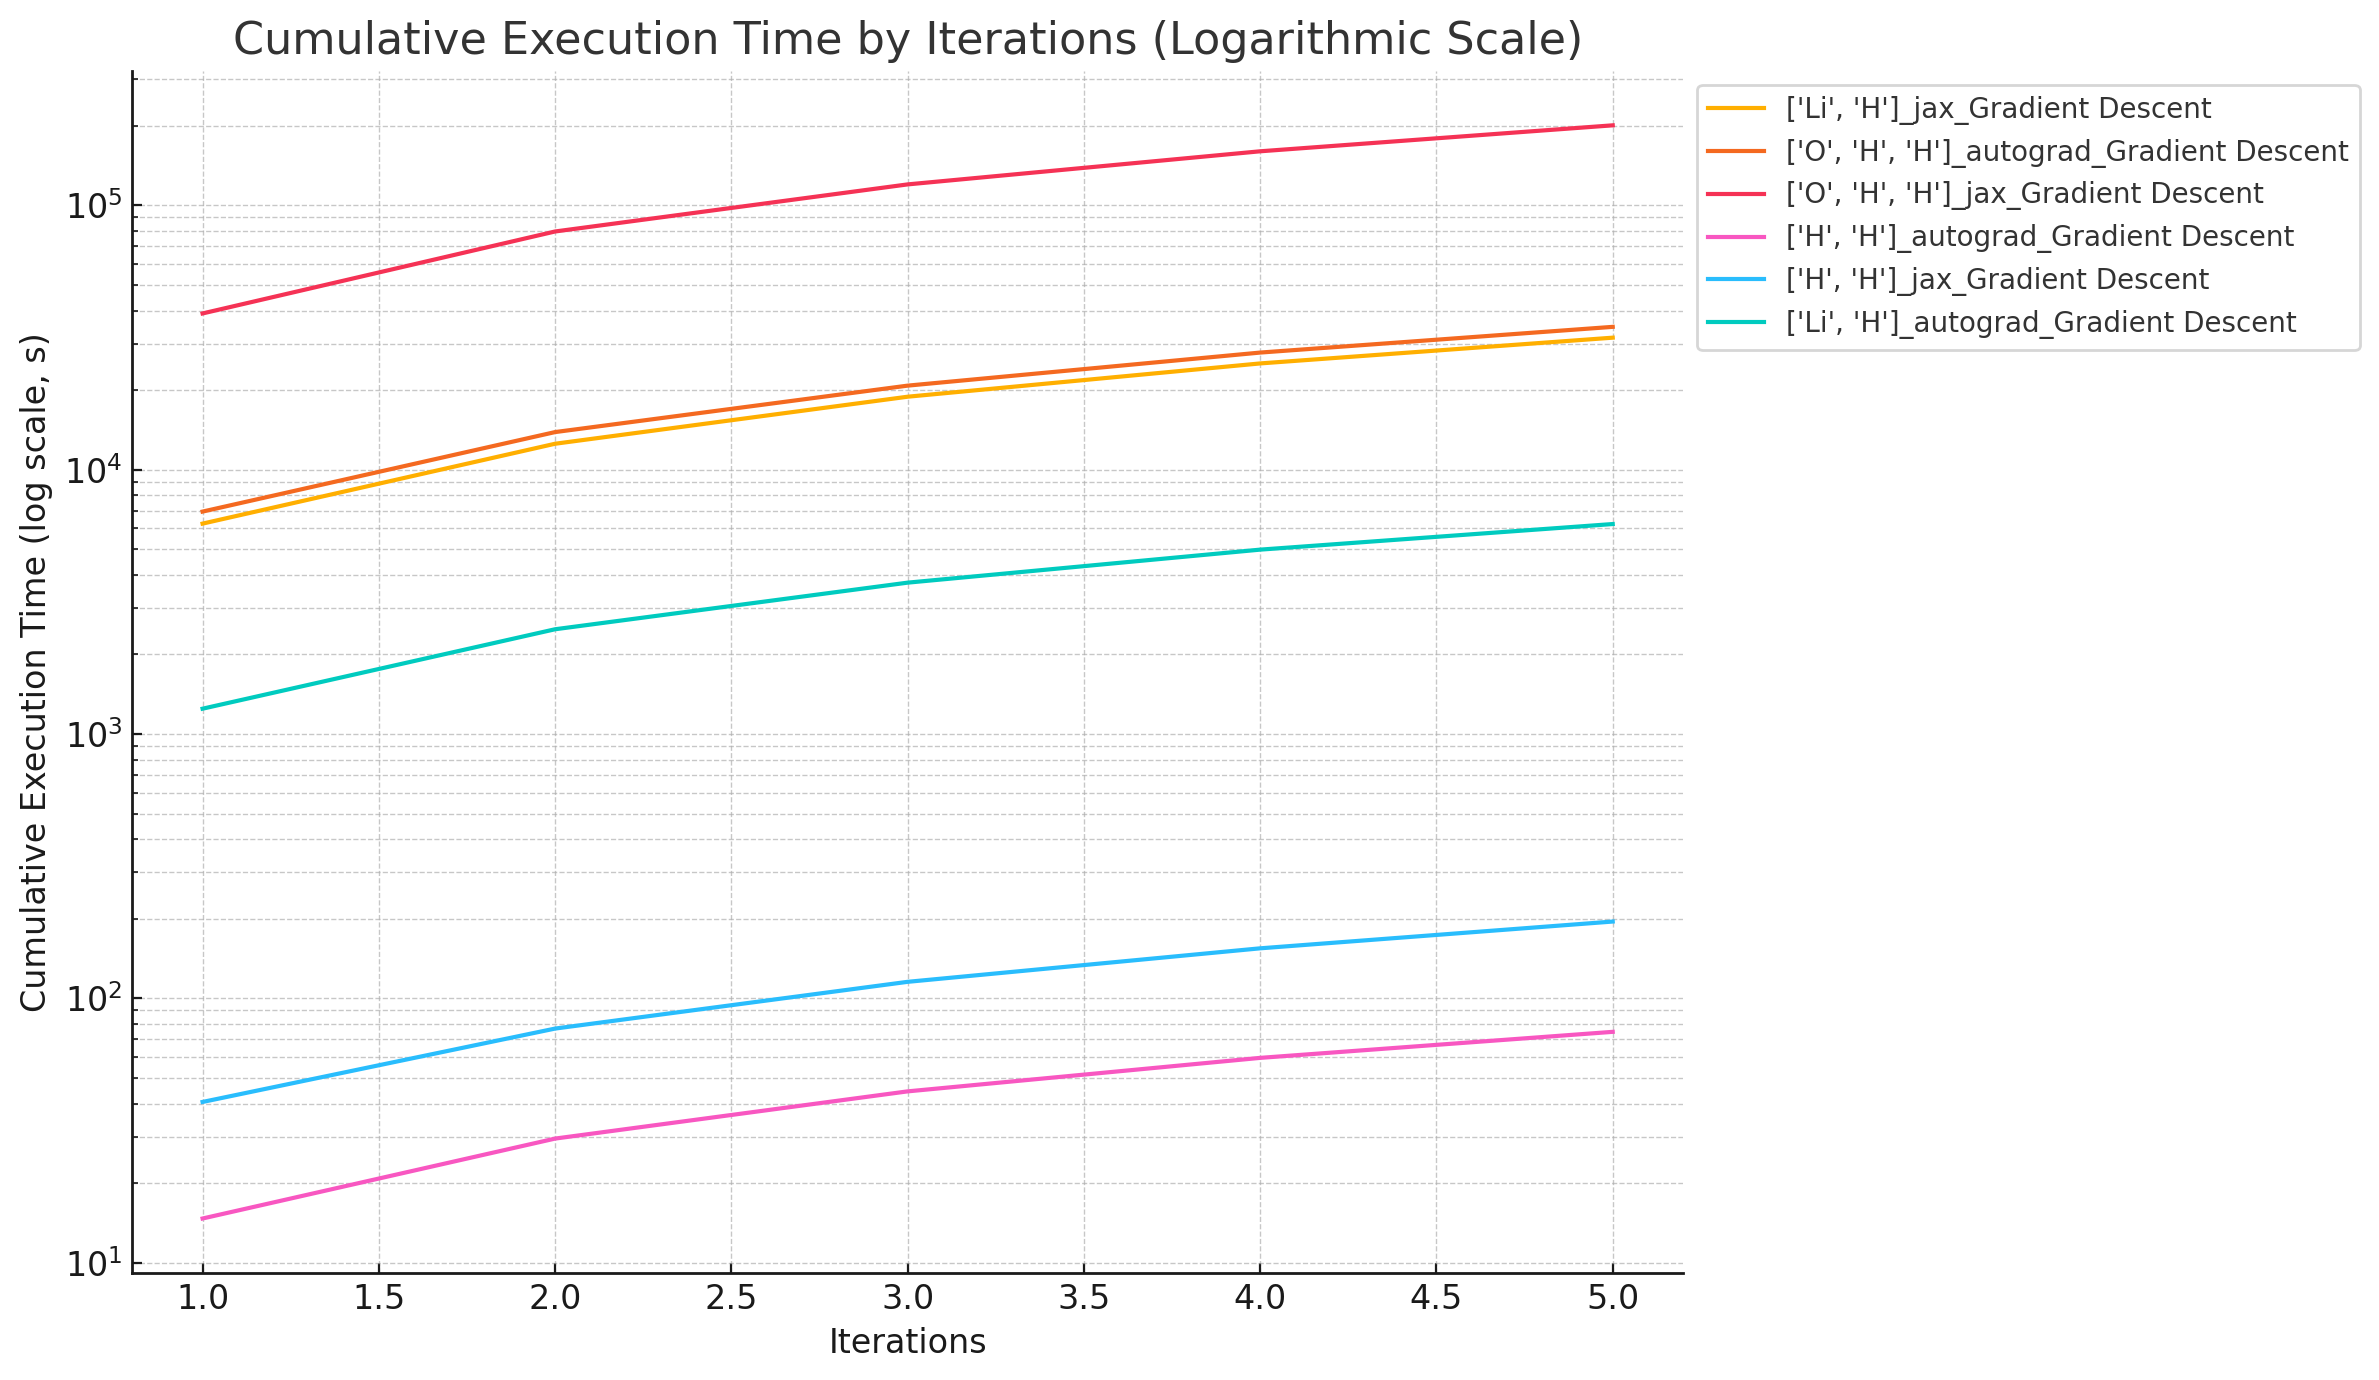
\includegraphics[width=0.8\textwidth]{img/time_iterations.png}
  \caption{Execution time of different molecules per iteration in the simulation.}
  \label{fig:time_iterations}
\end{figure}

\subsubsection{Comparative Performance Analysis}
To evaluate the performance of both interfaces in more detail, a table was created showing the percentage increase in execution time of \textit{JAX} compared to \textit{autograd}, as seen in Table~\ref{tab:jax_vs_auto}.

\begin{table}[H]
  \centering
  \scriptsize
  \resizebox{\textwidth}{!}{%
  \begin{tabular}{lcccc}
  \toprule
  \textbf{Metric} & 
  \textbf{LiH} & 
  \textbf{H\textsubscript{2}} & 
  \textbf{H\textsubscript{2}O} & 
  \textbf{Mean} \\
  \midrule
  \textbf{Total Time} & 80.28\% & 82.72\% & 61.75\% & 74.92\% \\
  \textbf{build\_hamiltonian} & 3.97\% & 8.49\% & 7.42\% & 6.63\% \\
  \textbf{compute\_operator\_gradients} & 91.24\% & 88.96\% & 94.70\% & 91.63\% \\
  \textbf{update\_parameters\_and\_coordinates} & 66.80\% & 74.62\% & 59.70\% & 67.04\% \\
  \bottomrule
  \end{tabular}%
  }
  \caption{Comparison of execution times between JAX and autograd interfaces for different molecules.}
  \label{tab:jax_vs_auto}
\end{table}

On average, it was observed that the \textit{JAX} interface exhibits a 74.92\% higher total execution time than the \textit{autograd} interface. Additionally, it is interesting to note that as the complexity of the molecule increases (with a greater number of atoms), the penalty percentage of \textit{JAX} tends to decrease. This behavior suggests that, in larger-scale problems, GPU acceleration could become more competitive, although it does not manage to outperform \textit{autograd} in this implementation.

\subsection{Computation Time per Function}
For a higher level of detail, the computation time was also measured for each part of the code where the interface change is introduced. Figure~\ref{fig:time_functions} shows the accumulated execution times in the main stages of the algorithm.

\begin{figure}[H]
  \centering
  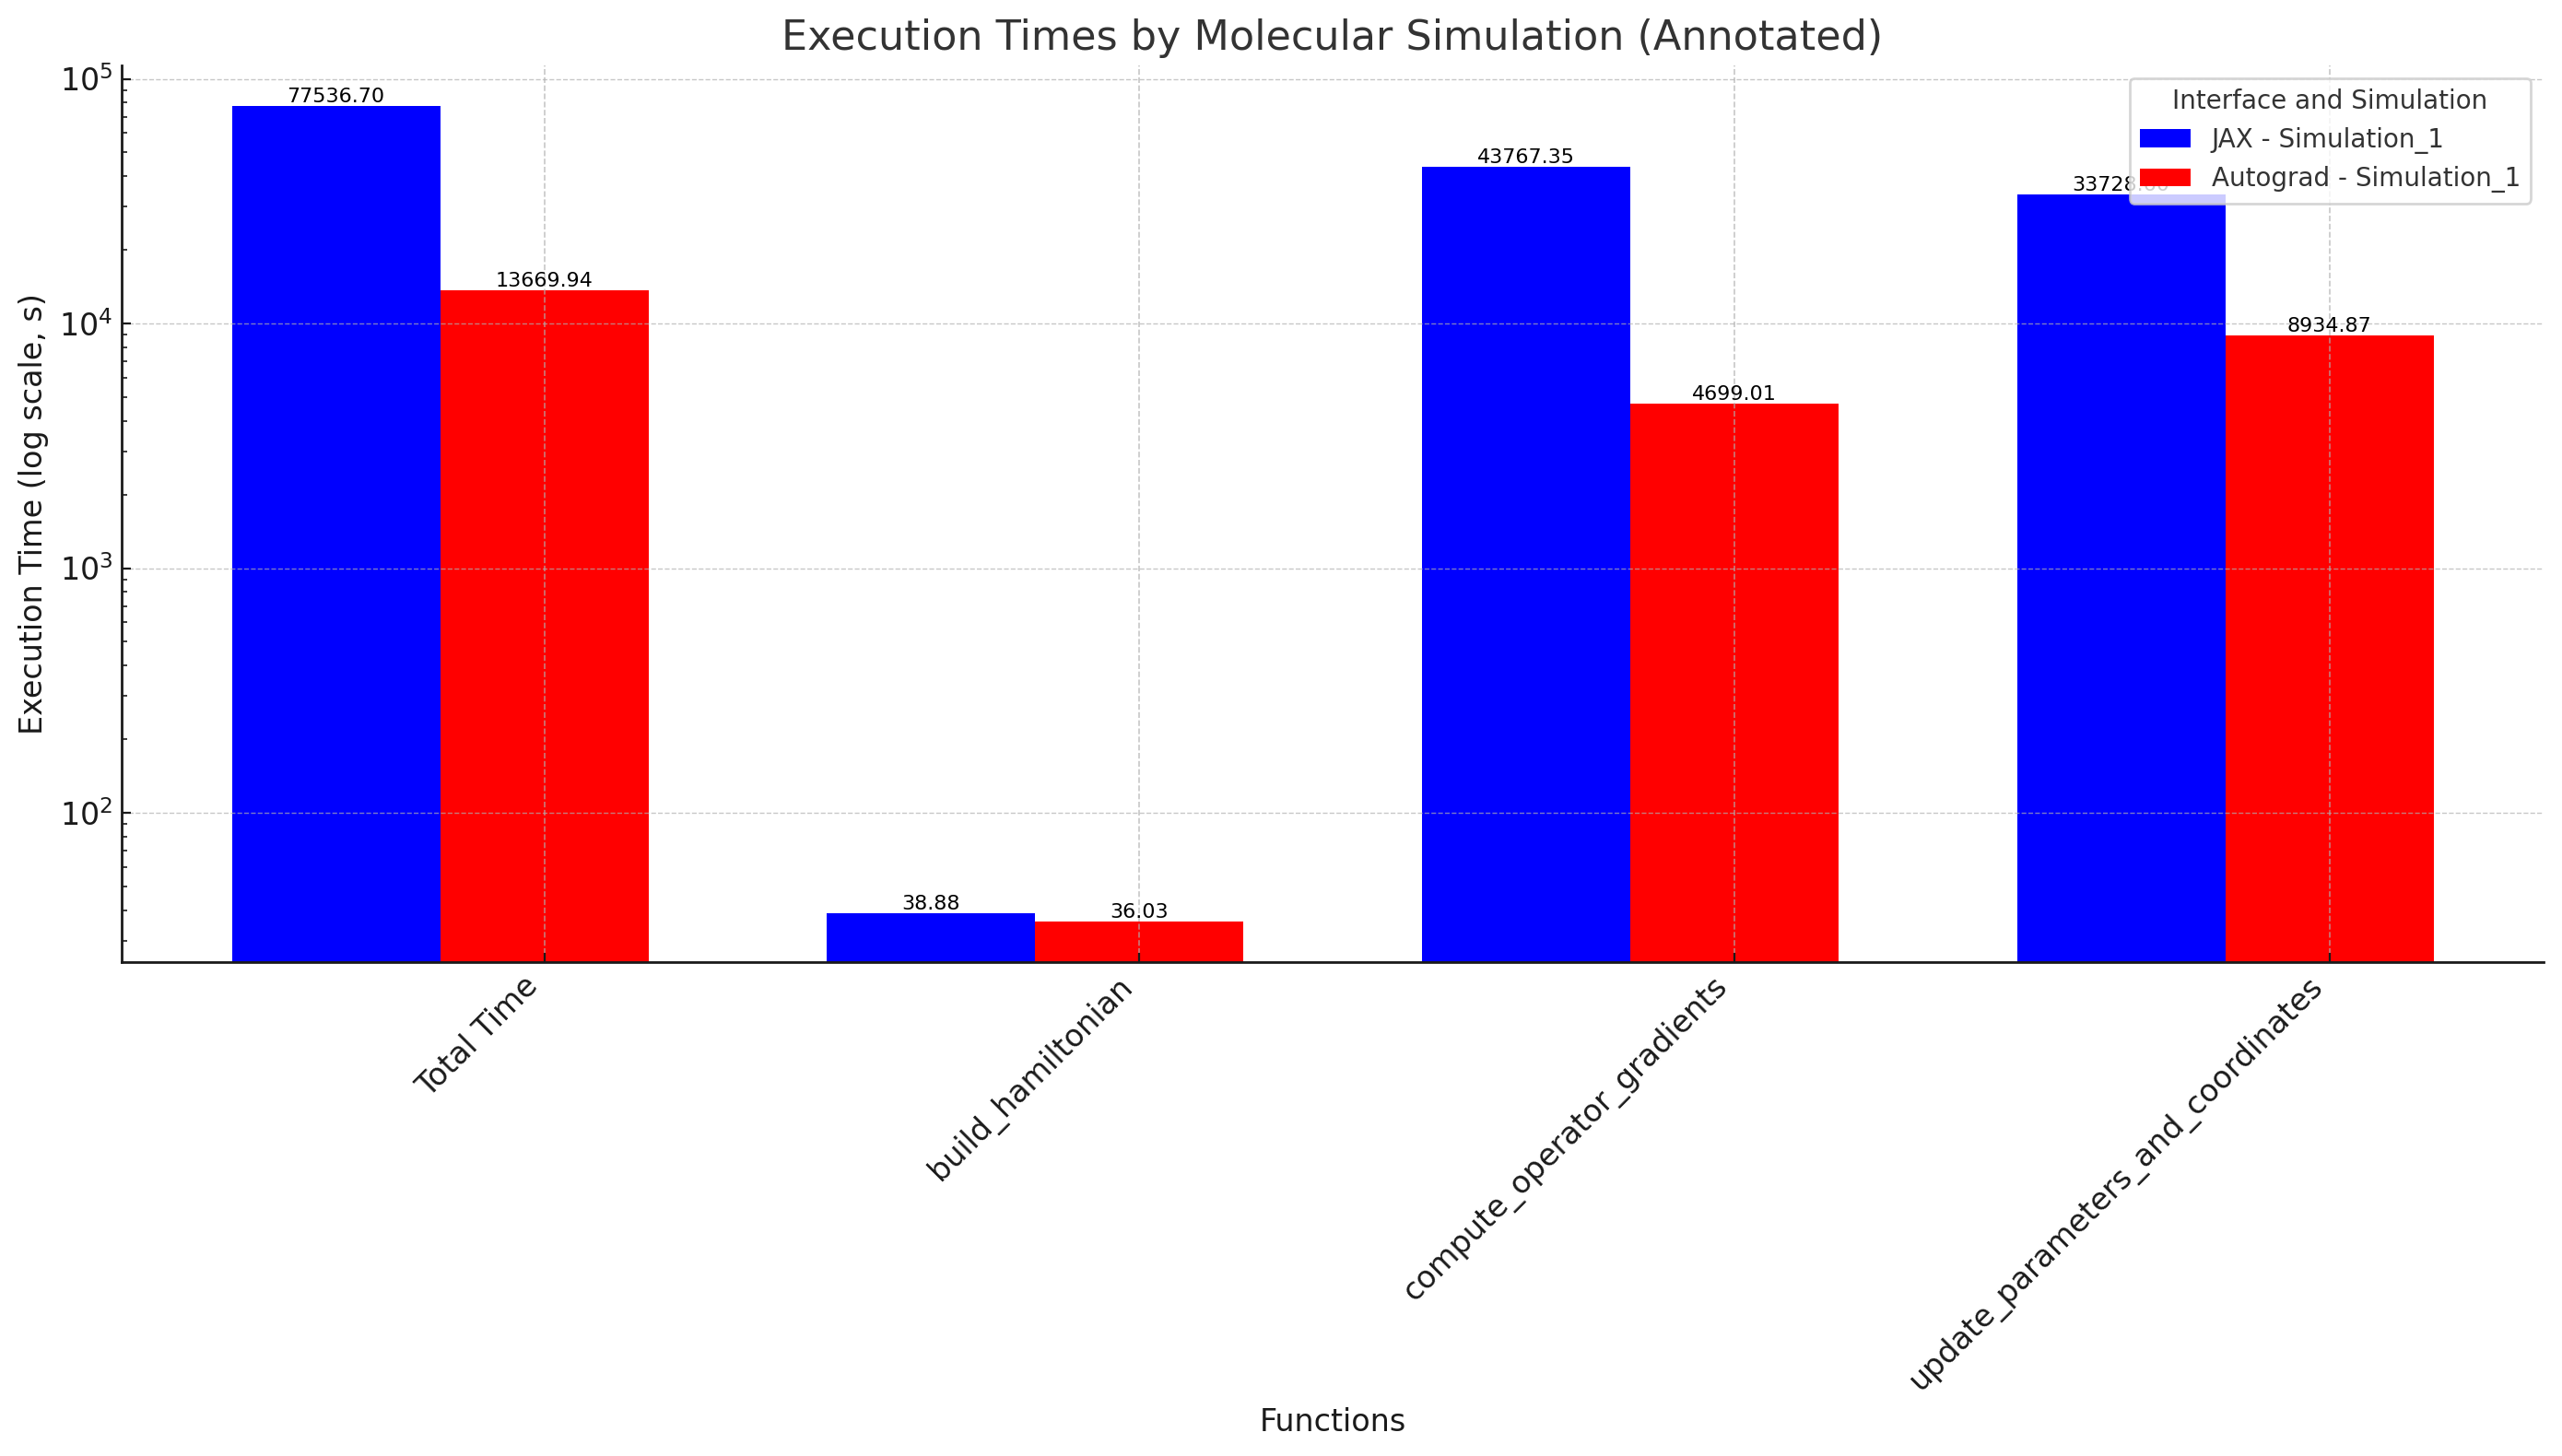
\includegraphics[width=0.8\textwidth]{img/time_functions.png}
  \caption{Execution time in different parts of the code.}
  \label{fig:time_functions}
\end{figure}

The same pattern is maintained in all functions: the \textit{JAX} interface records higher execution times than \textit{autograd}. In particular, the gradient computation part \texttt{compute\_operator\_gradients} increases its execution time by 91.68\% when using \textit{JAX}. This difference is largely attributed to the overhead caused by data transfer between the CPU and GPU, especially when \textit{PennyLane} does not fully support generating the molecule's Hamiltonian directly on the GPU.

On the other hand, the function \texttt{update\_parameters\_and\_coordinates}, responsible for performing the molecular geometry and parameter optimization step, also shows a 67.04\% increase when using \textit{JAX}. Nevertheless, it is worth highlighting that as the problem grows in complexity, the \textit{JAX} interface gains some relative efficiency in gradient calculation; however, the time saved through GPU acceleration is offset by the continuous data transfer between CPU and GPU throughout the iterations.

\subsection{Conclusions}
Based on the obtained results, the \textit{autograd} interface demonstrated superior performance in terms of speed for our implementation of the quantum molecular simulator. Although the GPU is usually advantageous in larger-scale problems, the data transfer overhead and the lack of full support for Hamiltonian generation within the GPU reduced the efficiency of \textit{JAX}. For this reason, we ultimately chose to use the \textit{autograd} interface for the final implementation of the quantum molecular simulator.

\section{Ansatz Comparison}
One of the most important modifications that has significantly affected our code and its functionality has been the choice of the Ansatz. Our proposal has been to implement UCCSD, an Ansatz typically used for this type of simulation, as it enhances the simulation performance by achieving higher efficiency. The efficacy of this type of Ansatz has already been demonstrated, showing how it can improve simulation performance by producing more optimal quantum circuits without the need to create a specific Ansatz for the molecule being simulated. It is a fact that for each optimizer configuration and for each different molecule simulation, there exists an optimal quantum circuit that achieves the best performance. However, since our objective is to develop a program that can simulate various molecules with maximum performance, we observe that the best option is UCCSD. To illustrate how our simulation performance is improved, we have generated Ansätze with different levels of depth and compared their performance with that of a UCCSD Ansatz. We have simulated various configurations of classical Ansätze, and in all cases, the UCCSD Ansatz has achieved better performance. More complex and molecule-specific Ansätze could be tested, but it is unlikely that another type of Ansatz would outperform UCCSD in terms of performance improvement.

Below is a simulation with different Ansatz depths and varying numbers of iterations obtained directly from the simulation.

\begin{figure}[H]
  \centering
  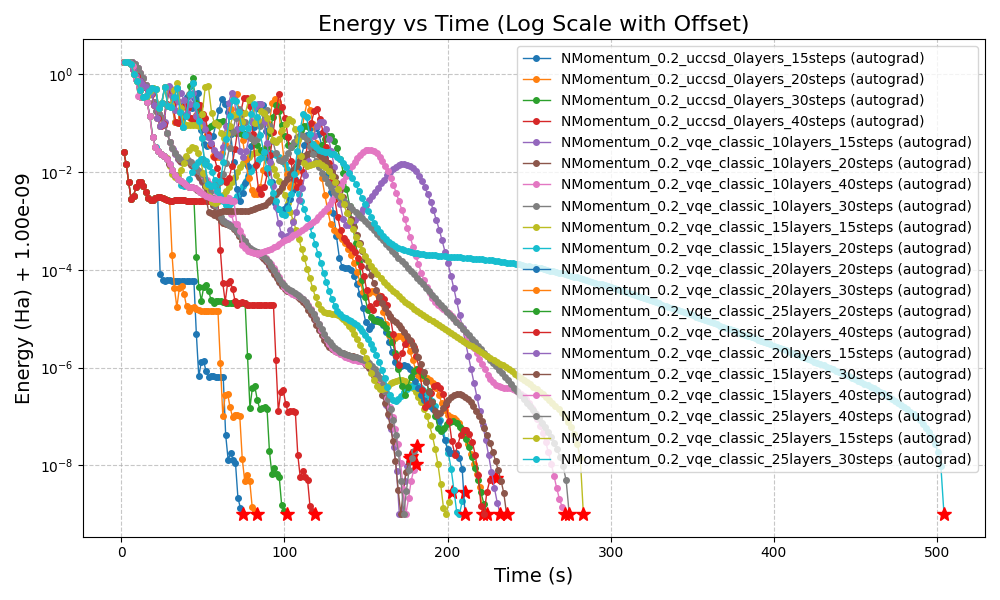
\includegraphics[width=0.8\textwidth]{data/Anzatz/results_ansatz_lyers_dif_iterations/energy_vs_time_log_offset.png}
  \caption{Energy vs. Time for different Ansätze and iterations.}
  \label{fig:ansatz_layers_iterations}
\end{figure}

It is observed that the UCCSD Ansatz achieves the best performance in all simulations, regardless of the number of optimizations performed for each iteration. For greater clarity of the results, a simulation was conducted with only a single number of optimizations per iteration, and the performance of the different Ansätze was compared, providing a clearer view of how UCCSD achieves the best performance.

\begin{figure}[H]
  \centering
  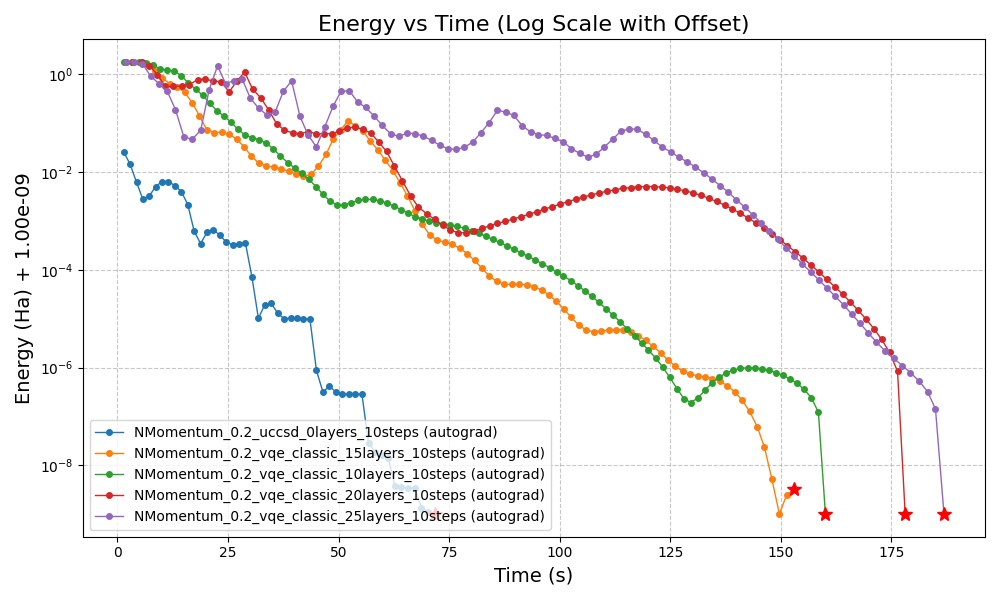
\includegraphics[width=0.8\textwidth]{data/Anzatz/results_ansatz_lyers/energy_vs_time_log_offset.png}
  \caption{Energy vs. Time for different Ansätze.}
  \label{fig:ansatz_layers}
\end{figure}

Finally, to corroborate that the UCCSD Ansatz achieves the best performance, a simulation was conducted with a different molecule, and the performance of the various Ansätze was compared. In the following image, it can be seen that the UCCSD Ansatz achieves the best performance in all simulations.

\section{Optimizer}

Once the Ansatz was selected, the next step was to choose and configure the optimizer. For this purpose, preliminary simulations were conducted to identify the best configuration.

\subsection{Optimizer Selection}
To determine the most effective optimizer for different molecules, a set of simulations was designed to analyze the evolution of energy as a function of iterations. To achieve this, we developed a procedure that allowed executing the same molecules with various optimizers, each covering a range of \emph{step size} values. This approach enabled the selection of the most appropriate \emph{step size} for each case.

In the first phase, which executed 42 processes in parallel, the \emph{step size} offering the best performance was observed for each optimizer and molecule. Subsequently, the simulation was repeated using only those optimal \emph{step sizes}. The results are shown below.

\begin{figure}[H]
  \centering
  % First image
  \begin{subfigure}{0.32\textwidth}
    \includegraphics[width=\textwidth]{data/Optimizadores/final_results_H2/energy_evolution_log_offset.png}
    \caption{H2 simulation.}
    \label{fig:subimage1}
  \end{subfigure}
  % Second image
  \begin{subfigure}{0.32\textwidth}
    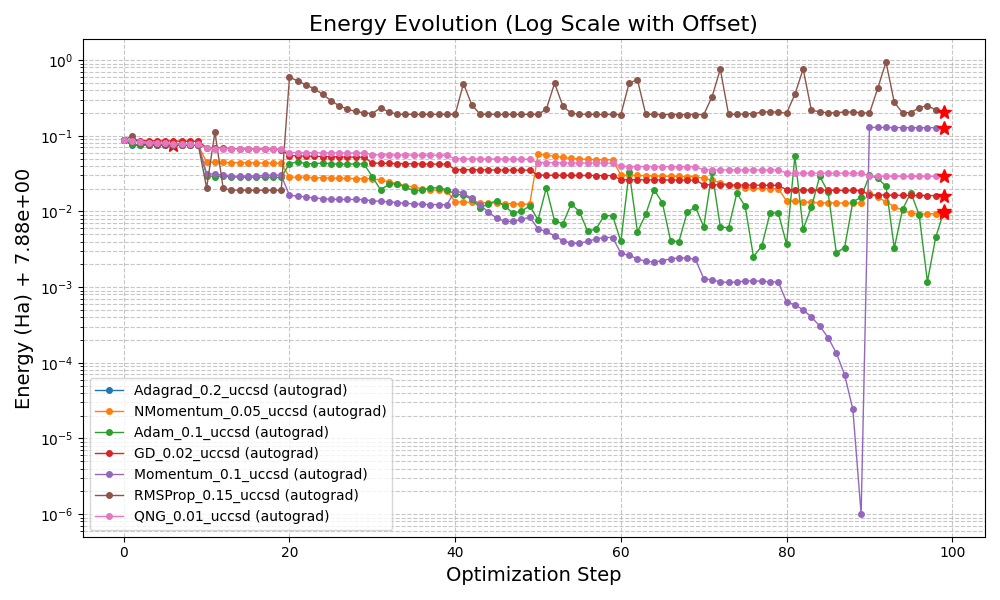
\includegraphics[width=\textwidth]{data/Optimizadores/final_results_LiH/energy_evolution_log_offset.png}
    \caption{LiH simulation.}
    \label{fig:subimage2}
  \end{subfigure}
  % Third image
  \begin{subfigure}{0.32\textwidth}
    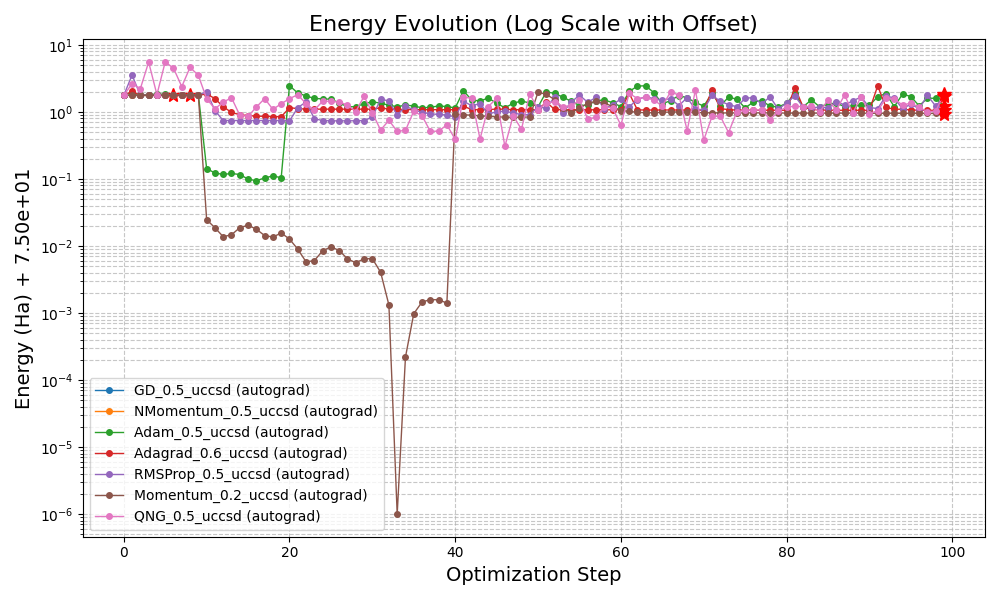
\includegraphics[width=\textwidth]{data/Optimizadores/final_results_H20/energy_evolution_log_offset.png}
    \caption{H2O simulation.}
    \label{fig:subimage3}
  \end{subfigure}
  \caption{Optimal \emph{step size} selection for each optimizer and molecule.}
  \label{fig:three_images}
\end{figure}

To delve deeper into the performance of the different optimizers, the following tables present the final energy, total optimization time, and the number of iterations required to converge for each molecule.

\subsubsection{Molecule \(\mathrm{H_2O}\)}

\begin{table}[H]
\centering
\caption{Final energy and optimization time for \(\mathrm{H_2O}\) (without using FCI).}
\begin{tabular}{lccc}
\toprule
\textbf{Optimizer} & \textbf{Final Energy (Ha)} & \textbf{Total Time (s)} & \textbf{Iterations} \\
\midrule
Adam (0.5)       & -73.75990609 & 28454.49 & 10 \\
Adagrad (0.6)    & -73.93046296 & 28891.08 & 10 \\
NMomentum (0.5)  & -73.22152796 & 7497.83  &  1 \\
Momentum (0.2)   & \textbf{-74.03997489} & 68420.47 & 10 \\
RMSProp (0.5)    & -73.28585876 & 65470.02 & 10 \\
GD (0.5)         & -73.22152796 & \textbf{6486.79}  &  1 \\
QNG (0.5)        & -73.13971041 & 70716.22 & 10 \\
\bottomrule
\end{tabular}
\end{table}

In this molecule, the most \emph{negative} energy is provided by \textbf{Momentum (0.2)}, with \(-74.03997489\)\,Ha, but at the cost of a very high time (68420.47\,s). On the other hand, \textbf{GD (0.5)} requires only 6486.79\,s, although its energy value \((-73.22152796)\,\mathrm{Ha}\) is somewhat less negative.

\subsubsection{Molecule \(\mathrm{H_2}\)}

\begin{table}[h!]
\centering
\caption{Final energy and optimization time for \(\mathrm{H_2}\).}
\begin{tabular}{lccc}
\toprule
\textbf{Optimizer} & \textbf{Final Energy (Ha)} & \textbf{Total Time (s)} & \textbf{Iterations} \\
\midrule
Adam (0.1)       & -1.07655292  & 173.30  & 10 \\
Adagrad (0.25)   & -1.13469066  & 10.19   &  1 \\
NMomentum (0.25) & -1.13730600  & 62.84   &  4 \\
Momentum (0.3)   & \textbf{-1.13730605} & 100.43  &  6 \\
RMSProp (0.1)    & -1.13675411  & 33.14   &  2 \\
GD (0.3)         & \textbf{-1.13730605} & 41.77   &  3 \\
QNG (0.1)        & -1.13469066  & 18.40   &  1 \\
\bottomrule
\end{tabular}
\end{table}

In this case, the most negative values (\(-1.13730605\)\,Ha) correspond to both \textbf{Momentum (0.3)} and \textbf{GD (0.3)}. If speed is a priority, \textbf{GD (0.3)} only requires 41.77\,s, making it a very competitive option.

\subsubsection{Molecule \(\mathrm{LiH}\)}

\begin{table}[H]
\centering
\caption{Final energy and optimization time for \(\mathrm{LiH}\).}
\begin{tabular}{lccc}
\toprule
\textbf{Optimizer} & \textbf{Final Energy (Ha)} & \textbf{Total Time (s)} & \textbf{Iterations} \\
\midrule
Adam (0.1)       & -7.87024707 & 13444.57 & 10 \\
Adagrad (0.2)    & -7.80548501 & 977.86   &  1 \\
NMomentum (0.05) & \textbf{-7.87085783} & 13442.59 & 10 \\
Momentum (0.1)   & -7.75267240 & 13566.98 & 10 \\
RMSProp (0.15)   & -7.67650000 & 13671.22 & 10 \\
GD (0.02)        & -7.86422129 & 13449.49 & 10 \\
QNG (0.01)       & -7.85120449 & 13776.00 & 10 \\
\bottomrule
\end{tabular}
\end{table}

Here, the lowest value \((-7.87085783)\,\mathrm{Ha}\) is achieved with \textbf{NMomentum (0.05)}. Both NMomentum (0.05) and Adam (0.1) surpass \(-7.870\)\,Ha with very similar times (both around 13400\,s). Meanwhile, \textbf{Momentum (0.1)} proves to be slower and less effective in terms of energy.

In summary, \emph{there is no universally optimal optimizer}. The choice depends on the molecule, acceptable computational cost, and the goal in terms of final energy. \textbf{Momentum} usually reaches the lowest values, although sometimes with high time requirements. \textbf{GD}, on the other hand, converges quickly and offers results close to the most negative minima in several tests. After reviewing the obtained results, we decided to choose the Momentum optimizer, as it achieves the best convergence without requiring excessive computation time.

\subsection{Step Size Selection}
To determine the most suitable \textit{step size} range, we started with the optimal value identified during optimizer selection. Subsequently, additional simulations were designed with values close to the initial optimum to refine this selection. This section presents the evolution of energy as a function of iterations, considering different \textit{step size} values for each molecule.

\begin{figure}[H]
  \centering
  % First image
  \begin{subfigure}{0.32\textwidth}
    \includegraphics[width=\textwidth]{data/StepSize/results_H2/energy_evolution_log_offset.png}
    \caption{H$_2$ simulation.}
    \label{fig:step_size_h2}
  \end{subfigure}
  % Second image
  \begin{subfigure}{0.32\textwidth}
    \includegraphics[width=\textwidth]{data/StepSize/results_LiH/energy_evolution_log_offset.png}
    \caption{LiH simulation.}
    \label{fig:step_size_lih}
  \end{subfigure}
  % Third image
  \begin{subfigure}{0.32\textwidth}
    \includegraphics[width=\textwidth]{data/StepSize/results_H2O/energy_evolution_log_offset.png}
    \caption{H$_2$O simulation.}
    \label{fig:step_size_h2o}
  \end{subfigure}
  \caption{Energy evolution as a function of \textit{step size} for different molecules.}
  \label{fig:step_size_results}
\end{figure}

Below, the final tables of energy, total optimization time, and the number of iterations for each molecule are shown. Note that in this case, each row corresponds to a \textit{step size}, keeping the same optimizer (in our case, \textbf{Momentum}).

\subsubsection{Molecule \(\mathrm{H_2}\)}

\begin{table}[H]
\centering
\caption{Final energy and optimization time for \(\mathrm{H_2}\) varying the \textit{step size} (optimizer: Momentum).}
\begin{tabular}{lccc}
\toprule
\textbf{Step Size} & \textbf{Final Energy (Ha)} & \textbf{Total Time (s)} & \textbf{Iterations} \\
\midrule
0.10 & \(\mathbf{-1.13730605}\) & 113.23 & 10 \\
0.12 & \(\mathbf{-1.13730605}\) & \(\mathbf{92.55}\) & 10 \\
0.14 & \(\mathbf{-1.13730605}\) & 131.52 & 10 \\
0.16 & \(\mathbf{-1.13730605}\) & 101.46 & 10 \\
0.18 & \(\mathbf{-1.13730605}\) & 149.96 & 10 \\
0.20 & -1.13730604 & 128.31 & 10 \\
0.22 & \(\mathbf{-1.13730605}\) & 111.54 & 10 \\
0.24 & \(\mathbf{-1.13730605}\) & 123.74 & 10 \\
0.26 & \(\mathbf{-1.13730605}\) & 115.02 & 10 \\
\bottomrule
\end{tabular}
\end{table}

In \(\mathrm{H_2}\), almost all \textit{step sizes} reach the same most negative energy \(\bigl(-1.13730605\,\mathrm{Ha}\bigr)\). If we prioritize speed, the \textit{step size} \(0.12\) is the most convenient, as it achieves this value in only \(92.55\,\mathrm{s}\).

\subsubsection{Molecule \(\mathrm{H_2O}\)}

\begin{table}[H]
\centering
\caption{Final energy and optimization time for \(\mathrm{H_2O}\) varying the \textit{step size} (optimizer: Momentum).}
\begin{tabular}{lccc}
\toprule
\textbf{Step Size} & \textbf{Final Energy (Ha)} & \textbf{Total Time (s)} & \textbf{Iterations} \\
\midrule
0.10 & \(\mathbf{-74.68985518}\) & 48577.15 & 10 \\
0.13 & -74.46832273 & 74175.94 & 10 \\
0.15 & -74.25355192 & 74211.21 & 10 \\
0.18 & -74.67526296 & 75127.97 & 10 \\
0.20 & -74.03997489 & 73130.72 & 10 \\
0.24 & -73.99558215 & 56465.58 & 10 \\
0.26 & -74.68963596 & \(\mathbf{44970.94}\) & 10 \\
0.28 & -74.59437540 & 75555.08 & 10 \\
0.30 & -74.65314486 & 73575.44 & 10 \\
\bottomrule
\end{tabular}
\end{table}

For \(\mathrm{H_2O}\), the \textit{step size} \(0.10\) offers the most negative energy \(\bigl(-74.68985518\,\mathrm{Ha}\bigr)\), while \(0.26\) notably reduces the total time to approximately \(44970.94\,\mathrm{s}\), with a very competitive energy value \(\bigl(-74.68963596\,\mathrm{Ha}\bigr)\).

\subsubsection{Molecule \(\mathrm{LiH}\)}

\begin{table}[H]
\centering
\caption{Final energy and optimization time for \(\mathrm{LiH}\) varying the \textit{step size} (optimizer: Momentum).}
\begin{tabular}{lccc}
\toprule
\textbf{Step Size} & \textbf{Final Energy (Ha)} & \textbf{Total Time (s)} & \textbf{Iterations} \\
\midrule
0.02 & -7.86678430 & \(\mathbf{13915.43}\) & 10 \\
0.04 & -7.87699744 & 14001.06 & 10 \\
0.06 & -7.88014045 & 13916.11 & 10 \\
0.08 & -7.87944832 & 14144.26 & 10 \\
0.10 & -7.75267240 & 14098.79 & 10 \\
0.12 & -7.87992395 & 13937.66 & 10 \\
0.14 & -7.78203292 & 14063.16 & 10 \\
0.16 & \(\mathbf{-7.88118152}\) & 13931.81 & 10 \\
0.18 & -7.88116774 & 13998.38 & 10 \\
\bottomrule
\end{tabular}
\end{table}

In \(\mathrm{LiH}\), the \textit{step size} \(0.16\) achieves the most negative final energy \(\bigl(-7.88118152\,\mathrm{Ha}\bigr)\). If the goal is to minimize computation time, the \textit{step size} \(0.02\) stands out with only \(13915.43\,\mathrm{s}\).

Thus, it is concluded that the choice of \textit{step size} depends both on the energy sought to be optimized and the acceptable computation time. For \(\mathrm{H_2}\), for example, a \textit{step size} of \(0.12\) achieves an excellent compromise between final energy and speed; whereas, for \(\mathrm{H_2O}\) and \(\mathrm{LiH}\), one might opt for values that minimize energy (case \(\mathrm{H_2O}\) with \(0.10\) and \(\mathrm{LiH}\) with \(0.16\)) or for shorter convergence times (for example, \(0.26\) in \(\mathrm{H_2O}\) and \(0.02\) in \(\mathrm{LiH}\)).

\section{Numero de Iteraciones}

Finalmente, una de los procesos donde mas tiempo se consume en la simulación es en la actualización de parametros y de las coordenadas, en esta ultima prueba lo que queremos conseguir es poder optimizar el numero de iteraciones que se actualizan los parametros y las coordenadas antes de volver a calcular el Hamiltoniano. Para ello, hemos generado una serie de simulaciones con distintos numeros de iteraciones, y hemos observado la evolución de la energia en función de las iteraciones. La configuarción de los optimizadores, han sido con los valores optimos que hemos obtenido despues de haber hecho todas las pruebas, con el optimizador Momentum y los valores de step size optimos.

\begin{figure}[H]
  \centering
  % First image
  \begin{subfigure}{0.45\textwidth}
    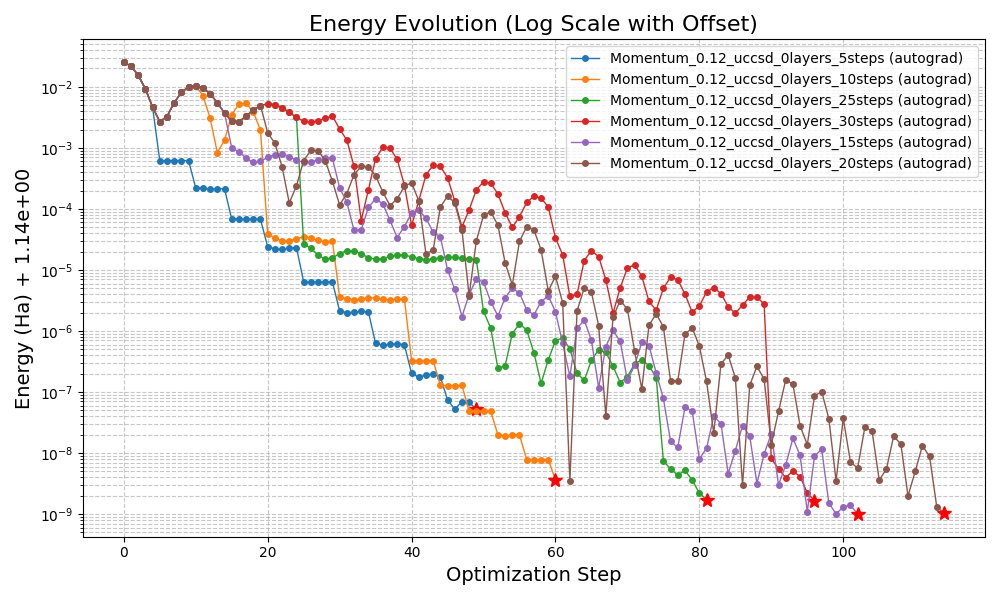
\includegraphics[width=\textwidth]{data/NumIterations/results_H2/energy_evolution_log_offset.png}
    \caption{H$_2$ simulation.}
    \label{fig:num_iterations_h2}
  \end{subfigure}
  % Second image
  \begin{subfigure}{0.45\textwidth}
    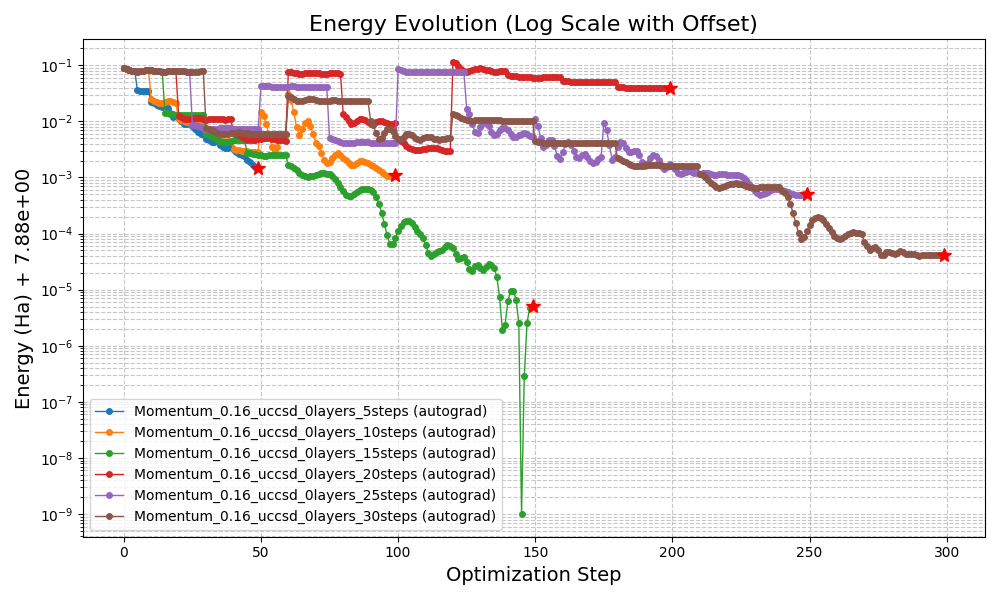
\includegraphics[width=\textwidth]{data/NumIterations/results_LiH/energy_evolution_log_offset.png}
    \caption{LiH simulation.}
    \label{fig:num_iterations_lih}
  \end{subfigure}
  % Third image
  \begin{subfigure}{0.45\textwidth}
    \includegraphics[width=\textwidth]{data/StepSize/results_H2O/energy_evolution_log_offset.png}
    \caption{H$_2$O simulation.}
    \label{fig:num_iterations_h2o}
  \end{subfigure}
  \caption{Energy evolution as a function of \textit{number of iterations} for different molecules.}
  \label{fig:num_iterations_results}
\end{figure}

Igual que en los apartados anteriores, a continuación mostramos las tablas con los valores de energia final, tiempo total de optimización y el numero de iteraciones necesarias para converger para cada molécula, para poder asi analizar los resultados obtenidos.

\subsubsection{Molecule \(\mathrm{H_2}\)}

\begin{table}[H]
\centering
\caption{Final energy and optimization time for \(\mathrm{H_2}\) using Momentum optimizer with varying steps.}
\begin{tabular}{lccc}
\toprule
\textbf{Steps} & \textbf{Final Energy (Ha)} & \textbf{Total Time (s)} & \textbf{Difference from FCI (Ha)} \\
\midrule
5 & \(\mathbf{-1.13730605}\) & 101.86 & -0.019800 \\ 
10 & \(\mathbf{-1.13730605}\) & \(\mathbf{99.08}\) & -0.019800 \\ 
15 & \(\mathbf{-1.13730605}\) & 163.25 & -0.019800 \\ 
20 & \(\mathbf{-1.13730605}\) & 175.06 & -0.019800 \\ 
25 & \(\mathbf{-1.13730605}\) & 124.58 & -0.019800 \\ 
30 & \(\mathbf{-1.13730605}\) & 147.59 & -0.019800 \\
\bottomrule
\end{tabular}
\end{table}

The most negative energy achieved for \(\mathrm{H_2}\) was \(-1.13730605\,\mathrm{Ha}\), with a difference from the exact FCI energy \(-1.117506\,\mathrm{Ha}\). Step counts of 10 provide an optimal trade-off between convergence speed and computational cost.

\subsubsection{Molecule \(\mathrm{LiH}\)}

\begin{table}[H]
\centering
\caption{Final energy and optimization time for \(\mathrm{LiH}\) using Momentum optimizer with varying steps.}
\begin{tabular}{lccc}
\toprule
\textbf{Steps} & \textbf{Final Energy (Ha)} & \textbf{Total Time (s)} & \textbf{Difference from FCI (Ha)} \\
\midrule
5 & \(-7.88079149\) & \(\mathbf{8328.30}\) & -0.017409 \\
10 & \(-7.88118152\) & 13365.38 & \(\mathbf{-0.017799}\) \\
15 & \(-7.88226478\) & 18384.78 & -0.018883 \\
20 & \(-7.84260017\) & 23309.87 & 0.020782 \\
25 & \(-7.88176386\) & 28433.90 & -0.018382 \\
30 & \(-7.88222895\) & 33421.15 & -0.018847 \\
\bottomrule
\end{tabular}
\end{table}

For \(\mathrm{LiH}\), the energy \(-7.88226478\,\mathrm{Ha}\) achieved in 15 steps shows the best accuracy compared to the FCI value \(-7.863382\,\mathrm{Ha}\), but the computation time is significantly lower for 5 steps (\(8328.30\,\mathrm{s}\)).

\subsubsection{Conclusions}

The results indicate that:
- For \(\mathrm{H_2}\), 10 steps balance speed and energy convergence.
- For \(\mathrm{LiH}\), 15 steps provide the most accurate energy, but fewer steps (5 or 10) can save substantial time with acceptable accuracy trade-offs.



\section{Limitations}
In the development of this project, several limitations have been identified that could have influenced the results obtained. It is essential to recognize and understand these limitations to properly interpret the conclusions and guide future research efforts.

\subsection{Availability of a Quantum Computer}
One of the most evident limitations has been the lack of access to a real quantum computer to validate the developed implementation. The simulation was conducted on classical hardware, which means it was not possible to directly verify how the simulator behaves on an actual quantum platform. This restriction limits the ability to evaluate the performance and efficiency of the implementation in a real quantum environment, where factors such as quantum coherence and entanglement could significantly influence the results.

\subsection{No Implementation of Quantum Errors}
Another significant limitation has been the absence of quantum error modeling in the simulation. In real quantum computers, errors arising from decoherence, imperfect quantum gates, and environmental noise are inevitable and can drastically affect the accuracy of simulations. By not incorporating these errors into the model, the simulation lacks the robustness required to faithfully reflect the operating conditions of a real quantum system. Including errors could have provided greater authenticity to the results, allowing for an evaluation of the simulator's resilience to the inherent imperfections of quantum computing.


